\section{Task 7: Automated Parameter Tuning - 2-Dimensional}

    \subsection{Task Description}
    Task 7 extends one-dimensional optimization to jointly optimize two interacting parameters of the Reverse Futility Pruning heuristic (\texttt{RFP\_intercept} and \texttt{RFP\_slope}) using two-dimensional Bayesian optimization. These parameters jointly determine the futility margin via $\text{margin} = \text{RFP\_intercept} + \text{RFP\_slope} \times \text{depth}$, requiring simultaneous optimization rather than sequential tuning.

  \subsection{Methodology}

  We employ 2D Bayesian optimization to jointly optimize \texttt{RFP\_intercept} and \texttt{RFP\_slope}, which determine the futility margin as:
  $\text{margin} = \text{RFP\_intercept} + \text{RFP\_slope} \times \text{depth}$.

  The optimization uses a Gaussian Process surrogate with separable bivariate Gaussian kernel:
  \begin{equation}
  k(\mathbf{x}, \mathbf{y}) = \sigma^2 \exp\left(-\frac{(x_1 - y_1)^2}{2l_1^2}\right) \exp\left(-\frac{(x_2 - y_2)^2}{2l_2^2}\right)
  \end{equation}

  The search space is $[-100, 300] \times [0, 500]$ subject to $\text{RFP\_intercept} + \text{RFP\_slope} > 0$, normalized to $[0,1]^2$ for numerical stability.

  \paragraph{Experimental Setup}
  We constructed a $5 \times 4$ factorial grid yielding 18 feasible configurations, evaluated via round-robin tournament (4,590 games, 15 positions, time control 30+0).
  Sequential iterations use Expected Improvement (EI) acquisition function with gauntlet evaluation (48 games per candidate against 4 diverse opponents). Fixed parameters:
  \texttt{NMP\_intercept}=3, \texttt{NMP\_slope}=0, \texttt{LMR\_intercept}=1, \texttt{LMR\_slope}=0.405.

  \subsection{Results}

  \paragraph{Initial Grid} Table~\ref{tab:task7_grid} shows top-10 configurations. Low slopes (0--167) dominate rankings; high slopes ($\geq 333$) consistently underperform.

  \begin{table}[H]
  \centering
  \caption{Top-10 initial configurations (18 total evaluated)}
  \label{tab:task7_grid}
  \begin{tabular}{rrccc}
  \hline
  \textbf{Rank} & \textbf{Intercept} & \textbf{Slope} & \textbf{Rating} & \textbf{SD} \\
  \hline
  1  & 100  & 167 & 2027.5 & 11.0 \\
  2  & 100  & 0   & 2027.3 & 11.4 \\
  3  & 0    & 167 & 2024.4 & 11.1 \\
  4  & 200  & 0   & 2020.1 & 11.3 \\
  5  & -100 & 167 & 2016.2 & 11.5 \\
  6  & 300  & 0   & 2015.2 & 11.2 \\
  7  & 200  & 167 & 2013.8 & 11.6 \\
  8  & 300  & 167 & 2009.9 & 11.4 \\
  9  & 200  & 333 & 2007.1 & 11.3 \\
  10 & 100  & 500 & 2001.1 & 11.5 \\
  \hline
  \end{tabular}
  \end{table}

  \paragraph{Sequential Optimization} Table~\ref{tab:sequential} summarizes iterations. Iteration 1 explored low-slope region, underperforming (providing negative evidence).
  Iteration 2 discovered superior configuration at intermediate slope. Iteration 3 auto-terminated due to low P(Improvement) = 0.21\%, indicating convergence.

  \begin{table}[H]
  \centering
  \caption{Sequential Bayesian optimization iterations}
  \label{tab:sequential}
  \begin{tabular}{ccccccc}
  \hline
  \textbf{Iter.} & \textbf{Intercept} & \textbf{Slope} & \textbf{Rating} & \textbf{SD} & \textbf{EI} & \textbf{P(Improv.)} \\
  \hline
  1 & 109 & 36  & 1943.4 & 38.0 & 0.0234 & 1.06\% \\
  2 & 100 & 69  & 2033.6 & 37.0 & 0.0386 & 1.63\% \\
  3 & 100 & 71  & ---    & ---  & 0.0041 & 0.21\% \\
  \hline
  \end{tabular}
  \end{table}

  \begin{figure}[H]
  \centering
  
\includegraphics[width=\textwidth]{media/iteration_0_2d.png}
  \caption{Initial Gaussian Process after 18-point factorial design. Left: GP posterior mean (predicted Elo). Center: GP posterior standard deviation (uncertainty). Right: Expected Improvement acquisition function. Red points indicate evaluated configurations.}
  \label{fig:gp_initial}
  \end{figure}

  \begin{figure}[H]
  \centering
  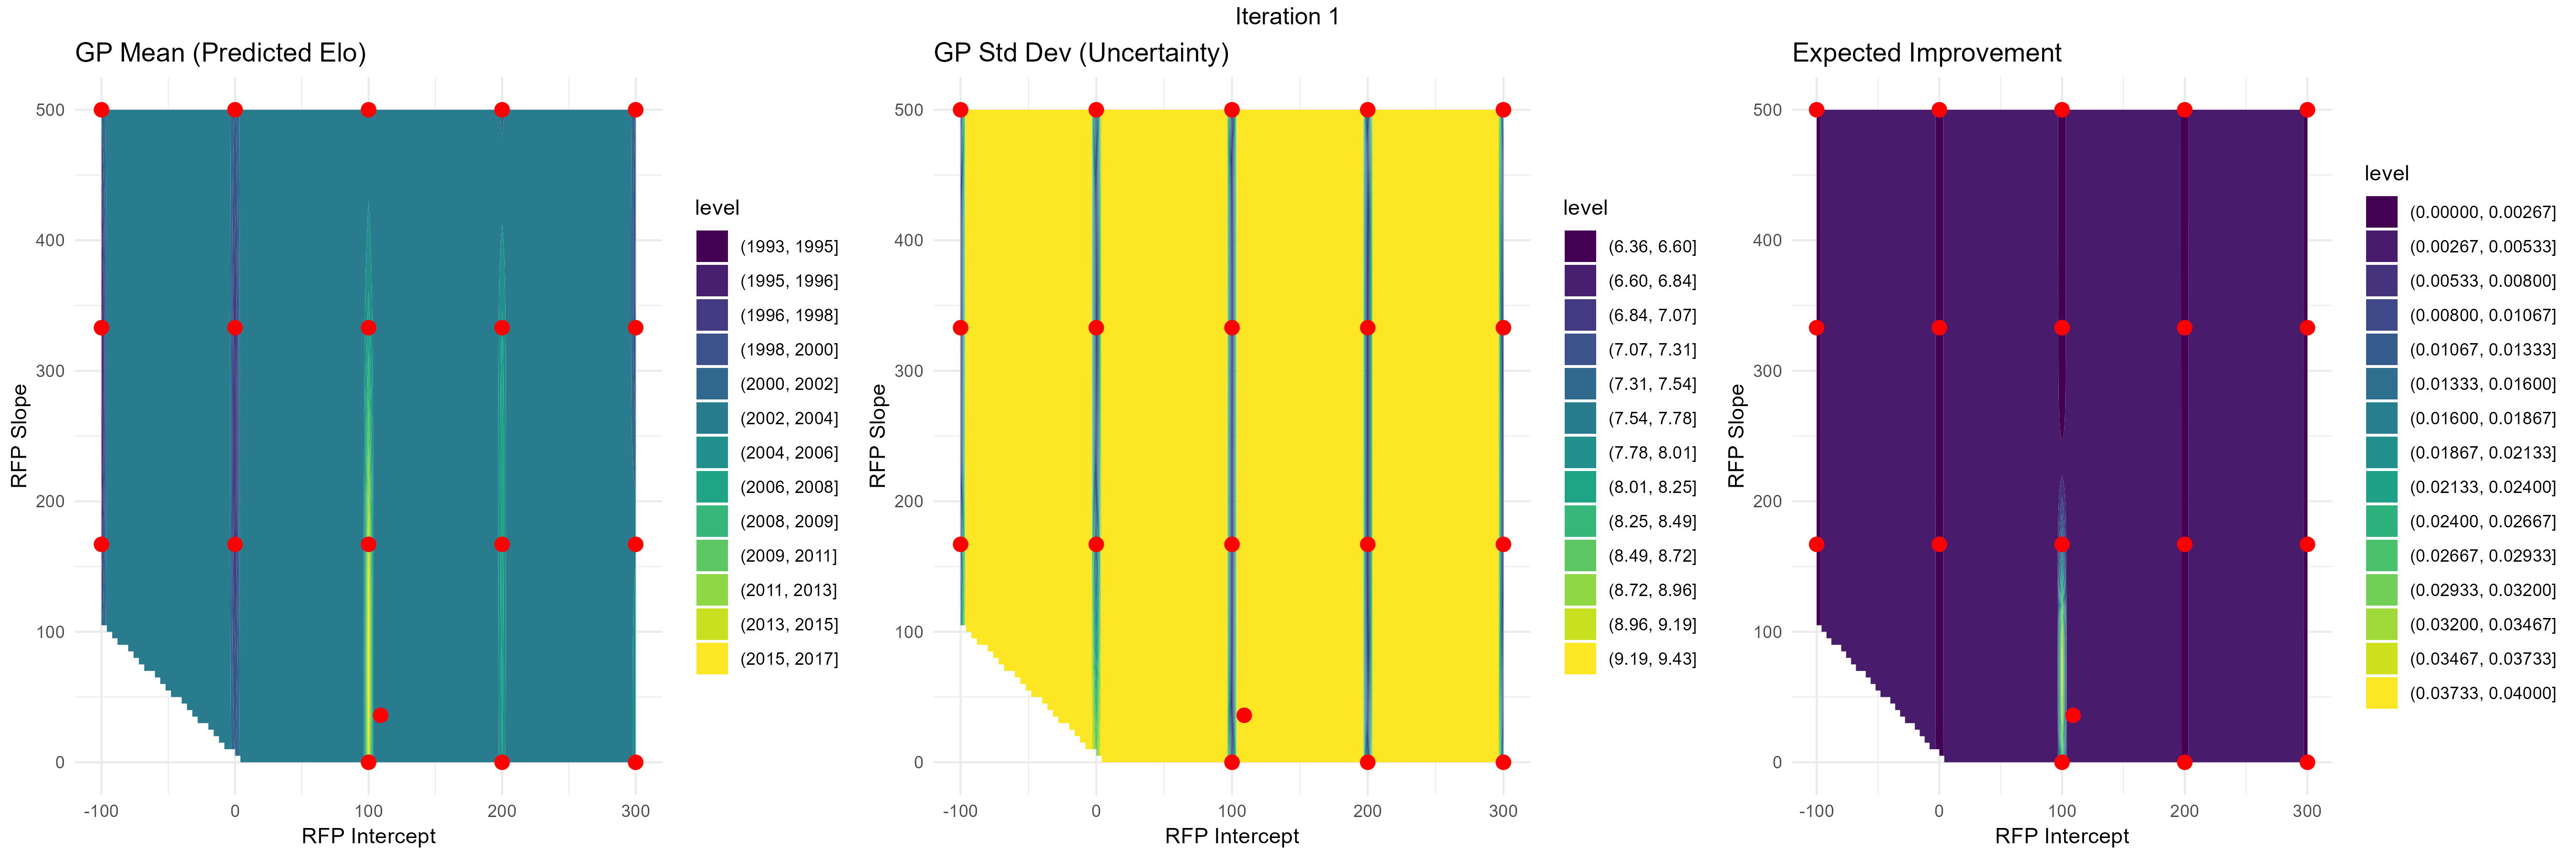
\includegraphics[width=\textwidth]{media/iteration_1_2d.png}
  \caption{Gaussian Process after first sequential iteration (19 total evaluations). The GP has been updated with the first candidate (intercept=109, slope=36) which underperformed, refining the posterior in the low-slope region.}
  \label{fig:gp_iter1}
  \end{figure}

  \begin{figure}[H]
  \centering
  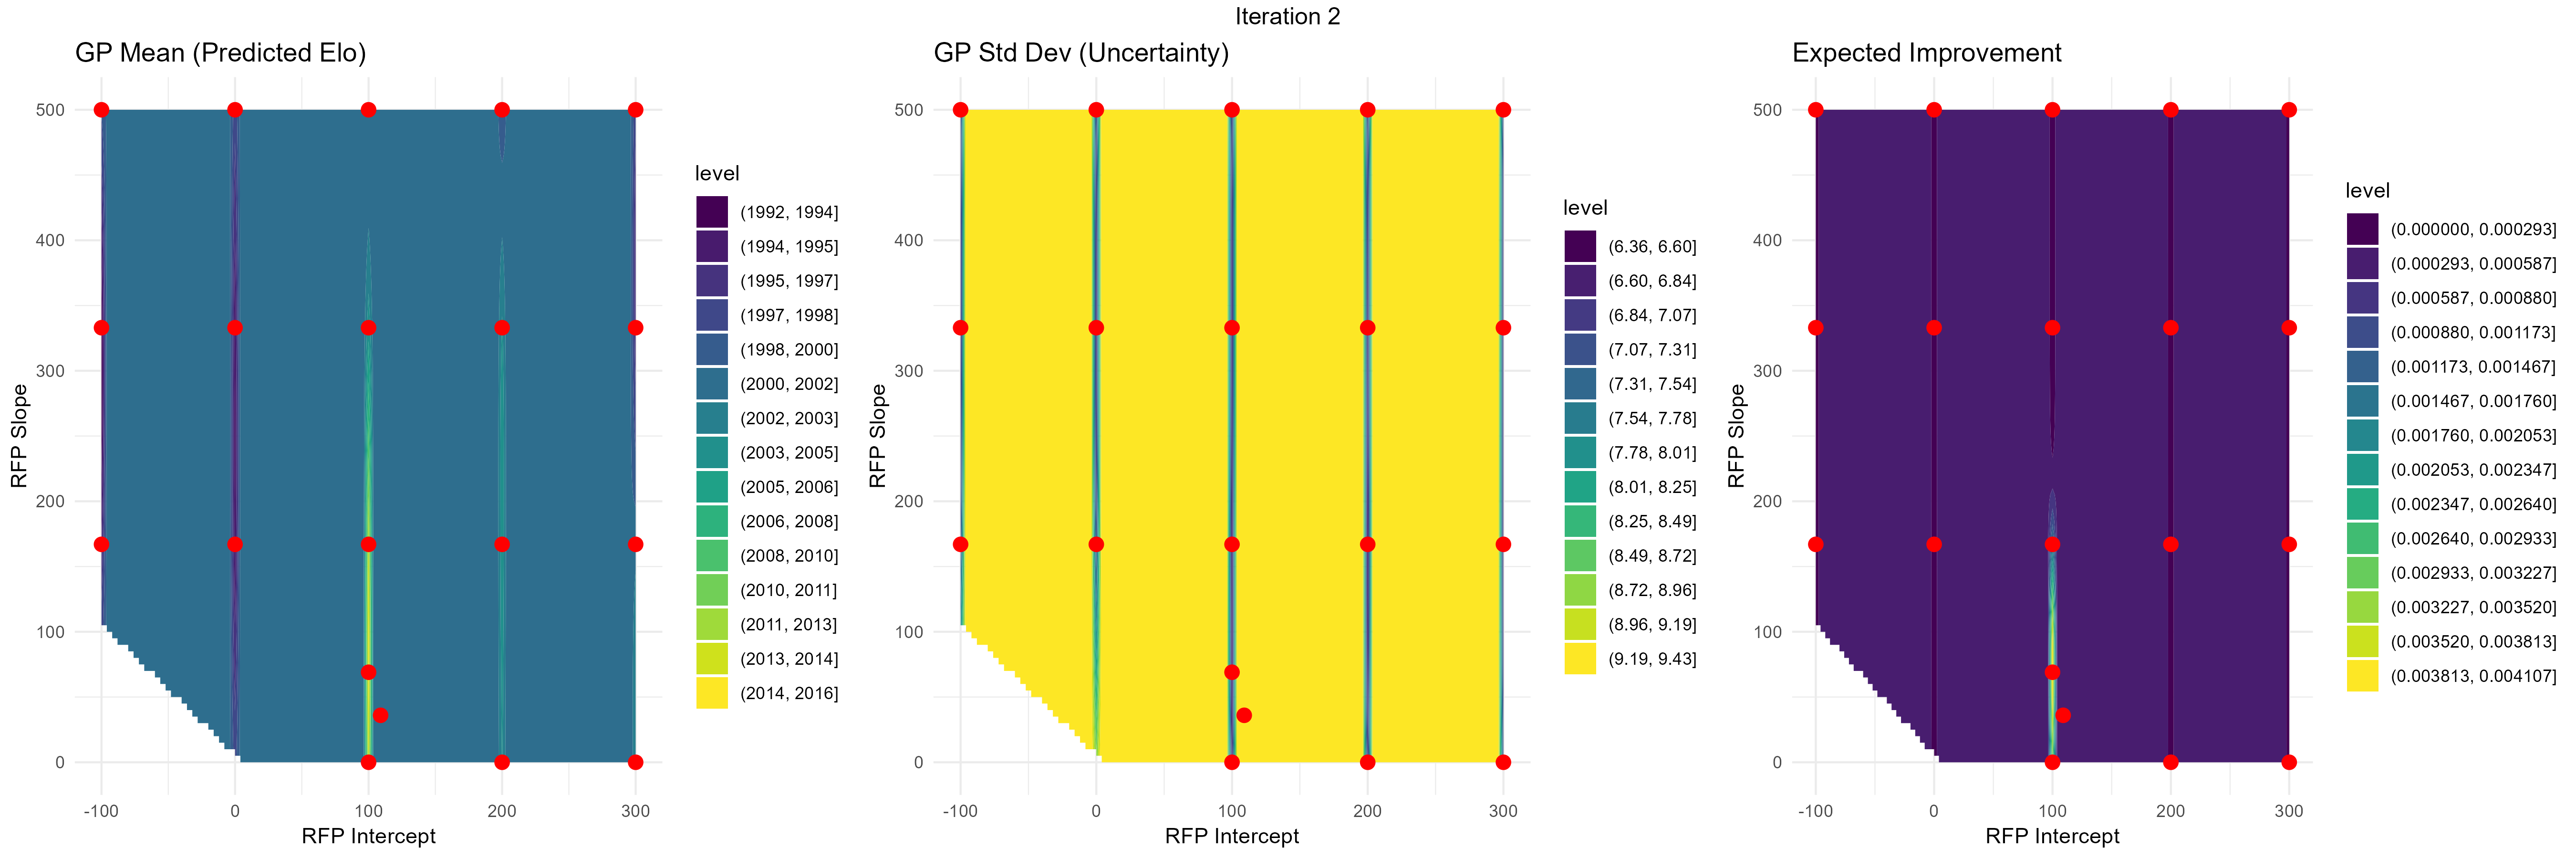
\includegraphics[width=\textwidth]{media/iteration_2_2d.png}
  \caption{Final Gaussian Process after 2 sequential Bayesian optimization iterations (20 total evaluations). The GP posterior shows refined mean estimates and substantially reduced uncertainty in the explored region around the optimum, with Expected Improvement concentrated in narrow bands indicating convergence.}
  \label{fig:gp_final}
  \end{figure}

  \paragraph{Optimal Parameters}
  Best configuration across 20 evaluations:
  \texttt{RFP\_intercept} = 100, \texttt{RFP\_slope} = 69, Elo = 2033.6 $\pm$ 37.0.
  This improves ~6 Elo over initial grid optimum (intercept=100, slope=167), demonstrating value of exploring intermediate regions between coarse grid points.

  \subsection{Conclusion}

  The 2D Bayesian optimization efficiently explored the constrained parameter space using 20 total evaluations (18 initial + 2 sequential), converging after detecting
  low improvement probability. Key findings:
  \begin{itemize}
      \item Moderate depth-scaling (slope $\approx$ 69) outperforms both depth-independent (slope=0) and coarser grid point (slope=167)
      \item High slopes ($\geq 333$) severely degrade performance due to excessive pruning at depth
      \item Optimal margin: 100 + 69 $\times$ depth centipawns
      \item Sequential exploration improved upon factorial grid by 6 Elo points
  \end{itemize}

  \textbf{Complete optimized parameters:} \texttt{NMP\_intercept}=3, \texttt{NMP\_slope}=0, \texttt{LMR\_intercept}=1, \texttt{LMR\_slope}=0.405,
  \texttt{RFP\_intercept}=100, \texttt{RFP\_slope}=69.